\question Q1\droppoints

\begin{solution}
    \text{(1)} Consider
    \[
        \mathcal{L(\mathbf{x}, \lambda)} = f(x) - \lambda(x_1^2 + x^2 - 1) = (8-\lambda)x_1^2 - \lambda x_2^2 - 2x^2 + \lambda
    \]

    Find the partial derivatives:

    \begin{equation*}
        \begin{cases}
            \frac{\partial \mathcal{L}}{\partial x_1} = 2(8 - \lambda)x_1 \\
            \frac{\partial \mathcal{L}}{\partial x_2} = -2\lambda x_2 - 2 \\
            \frac{\partial \mathcal{L}}{\partial \lambda} = x_1^2 + x_2^2 - 1 \\
        \end{cases}\label{eq:1}
    \end{equation*}

    Set them to zero, we obtain the following equation system:

    \begin{equation*}
        \begin{cases}
            2(8 - \lambda) x_ 1 = 0 \\
            \lambda x_2 = -1 \\
            x_1^2 + x_2^2 = 1
        \end{cases}\label{eq:2}
    \end{equation*}

    Case 1: When $(8 - \lambda) = 0$, we have:

    \begin{equation*}
        \begin{cases}
            x_1 = \pm \frac{3\sqrt{7}}{8} \\
            x_2 = -\frac{1}{8} \\
            \lambda = 8
        \end{cases}\label{eq:3}
    \end{equation*}

    Case 2: When $x_1 = 0$, we have:

    \begin{equation*}
        \begin{array}{c}
            \begin{cases}
                x_1 = 0 \\
                x_2 = 1 \\
                \lambda = -1
            \end{cases}
            \quad \text{or} \quad
            \begin{cases}
                x_1 = 0 \\
                x_2 = -1 \\
                \lambda = 1
            \end{cases}
        \end{array}
    \end{equation*}

    Therefore, we have four different points that reaches relative extrema:

    \[
        \mathbf{x}_1 =
        \begin{bmatrix}
            \frac{3\sqrt{7}}{8} \\ -\frac{1}{8}
        \end{bmatrix}
        \quad
        \mathbf{x}_2 =
        \begin{bmatrix}
            -\frac{3\sqrt{7}}{8} \\ -\frac{1}{8}
        \end{bmatrix}
        \quad
        \mathbf{x}_3 =
        \begin{bmatrix}
            0 \\ 1
        \end{bmatrix}
        \quad
        \mathbf{x}_4 =
        \begin{bmatrix}
            0 \\ -1
        \end{bmatrix}
    \]

    We verify each of them:

    \[
        \begin{align*}
            f(\mathbf{x}_1) &= 8\left(\frac{3\sqrt{7}}{8}\right)^2 -2\left(-\frac{1}{8}\right) = \frac{65}{8} \\
            f(\mathbf{x}_2) &= 8\left(-\frac{3\sqrt{7}}{8}\right)^2 -2\left(-\frac{1}{8}\right) = \frac{65}{8} \\
            f(\mathbf{x}_3) &= 8(0)^2 - 2(1) = -2 \\
            f(\mathbf{x}_3) &= 8(0)^2 - 2(-1) = 2 \\
        \end{align*}
    \]

    In conclusion, when subjecting to $x_1^2 + x_2^2 = 1$, $f(\mathbf{x})$ reaches the minimum value $-2$ at $(0, 1)^T$

    \text{(2)} Implemented in \textbf{question1.py}.
    The plot is as follows:

    \centerline {
        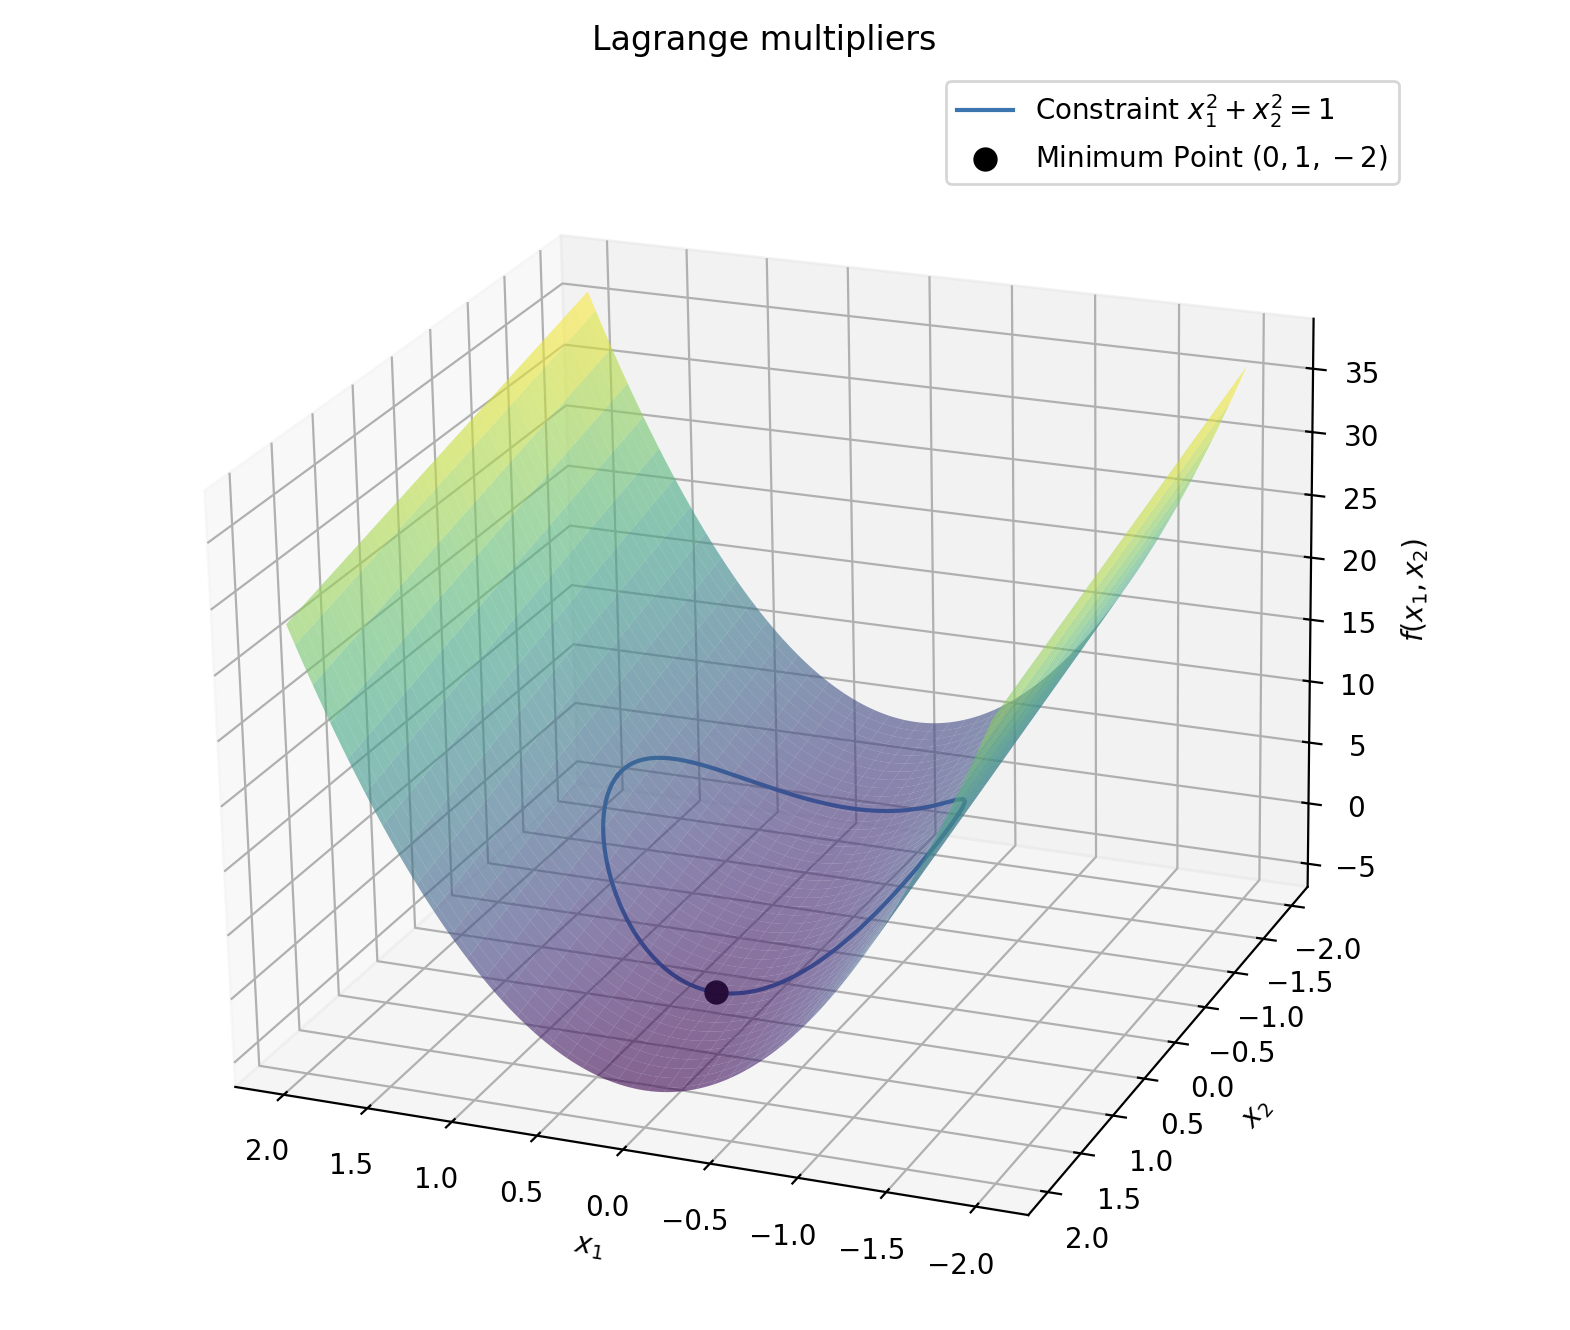
\includegraphics[width=1\textwidth]{img/q1}
    }

\end{solution}